\chapter{引言}
\section{选题背景及意义}
无网格法\cite{belytschkoMeshlessMethodsOverview1996b,chen2017,zhang2009,liu2009,wang2021b}是一类根据离散节点位置信息直接建立形函数的方法,其形函数具有高阶光滑的特点。相较于传统有限元法\cite{hughes2000, 2014Computer},形函数构造过程中不依赖网格信息,适用于复杂区域的离散,能有效减轻网格畸变所引起的计算精度下降的问题。依据这些特点,近二十年来无网格法得到了广泛的关注,发展出各种各具特色的无网格法。其中,包括基于强形式的配点型无网格法,
如光滑水动力学法\cite{1977A}、最小二乘配点法\cite{zhang2001}、再生梯度配点法\cite{chi2013}、自由单元法\cite{GaoXiaoWei2019}、再生核稳定配点法\cite{wang2020c}、超收敛无网格配点法\cite{deng2023}、加权径向基配点法\cite{xue2024}、彼得罗夫稳定配点法\cite{wang2022b}等,和基于弱形式的伽辽金型无网格法,
如无单元伽辽金法\cite{belytschko1994}、再生核粒子法\cite{liu1995}、单位分解法\cite{babuska1997}、自然单元法\cite{sukumar1998}、局部皮德罗夫伽辽金法\cite{long2002}、物质点法\cite{LianYanPing2013}、复变再生核无网格法\cite{ChengYuMin2005}、最大熵近似\cite{millan2011}、移动Kriging无网格法\cite{thai2016}、有限球法\cite{de2001}、广义有限元法\cite{strouboulis2001}、协调核函数无网格法\cite{koester2019}等。
无网格法也被应用于各类问题的分析中,如高阶薄板壳问题\cite{chen2015,deng2019,hilali2022,truong2024}、裂纹扩展问题\cite{GaoXin2018,zhu2021,nguyen2024}、动力分析问题\cite{ChenJian2022}、极端变形问题\cite{ZhangXiong2017,yreux2017}、声波传播问题\cite{you2024}等。
本论文讨论的是具有变分一致性的伽辽金无网格法\cite{chen2001,WuJunChao2016}。无网格法由于形函数及其梯度通常为有理式,在采用伽辽金法进行求解的时候,传统基于多项式完备性建立的高斯积分法无法进行准确数值积分过程,导致伽辽金无网格法无法准确求解与其基函数阶次相同的解析解,即不满足变分一致性\cite{1999Numerical, babuska2008, wu2021}。为了解决该问题,建立具有变分一致性的伽辽金无网格法成为无网格研究领域的热门问题。目前具有变分一致型的伽辽金无网格法主要是通过假定应变理论构造匹配的光滑梯度,光滑梯度为低阶多项式,采用低阶高斯积分法既能准确进行数值积分,保证计算误差的收敛阶次。同时,光滑梯度的构造过程仅需要计算传统无网格形函数,避免复杂耗时的形函数梯度计算,提高传统伽辽金无网格法的计算效率\cite{nguyen2008,nagevadiya2019}。然而,变分一致型伽辽金无网格法还存在以下问题:

变分一致型伽辽金无网格法目前的变分理论基础还是基于传统势能泛函,在进行该方法的误差估计过程仅简单地将传统无网格形函数导数替换乘光滑梯度表示\cite{wu2021}。光滑梯度并不等同于传统形函数导数,变分理论基础不够完备。完善变分一致型伽辽金无网格法的变分理论基础,将有助于对该方法进行精确的理论误差估计,利于方法后续的推广和使用。

具有变分一致性的无网格数值积分方案需要采用相同具有变分一致性的本质边界条件施加方案与之相配合,以满足全域变分一致性\cite{wang2016}。目前最常用于变分一致型伽辽金无网格法的本质边界条件施加方案为Nitsche法,该方法可是为拉格朗日乘子法与罚函数法相结合。Nitsche法修正拉格朗日乘子法中的乘子依据其实际物理意义采用位移进行表示,以保证变分一致性。然后,修正的变分一致项会导致整体刚度无法满足正定性,需要引入稳定项以得到满足要求的求解精度。Nitsche法采用罚函数法作为稳定项,罚函数法中存在人工经验参数,人工经验参数的大小直接影响计算精度。如图\ref{nitschepenalty}所示为变分一致型无网格数值积分方案(再生光滑梯度积分法RKGSI)配合罚函数法与Nitsche法的人工参数敏感性分析,图中颜色深浅代表不同疏密的离散模型,越深代表无网格节点越密集,越浅则无网格节点越稀疏。从结果可以看出,虽然Nitsche法相较于罚函数对人工参数的敏感性较低,但最优与最差的误差也相差了两个数量级。同时,最优人工参数的取值范围也与无网格节点疏密程度相关,不便于实际工程应用。

\begin{figure}[ht!]
\centering
    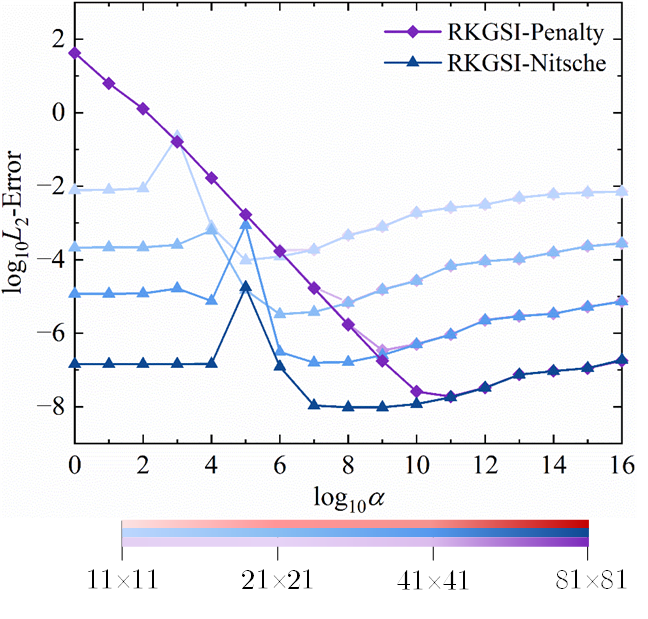
\includegraphics[scale=0.5]{figure/fig1.png}
    \caption{罚函数法与Nitsche法人工参数敏感性分析}\label{nitschepenalty}
\end{figure}

\section{国内外研究历史及现状}

变分一致型伽辽金无网格法可追溯到2004年Chen等人\cite{chen2001}提出的稳定节点积分法,该方法从伽辽金法的线性准确性条件出发,提出了线性积分条件。伽辽金数值积分方法需要从满足积分约束条件,才能准确求解线性问题,即满足线性的变分一致性。该方法以假定应变理论将背景积分域上的应变假设为常数,并命名此应变为光滑应变,通过满足线性积分约束条件确定光滑应变。该过程避免了求解耗时传统无网格形函数的导数,并将域内积分转化为边界积分,计算效率由于传统高斯积分法。
段庆林等人\cite{duan2012, duan2014}将线性积分约束条件推广至高阶情况,通过满足高阶积分约束条件以求解高斯积分点出的无网格光滑梯度。该方法以其高阶的变分一致性进一步被推广至薄板弯曲\cite{WangBingBing2019}和四阶相场\cite{shao2024}等高阶问题。但该一致性积分法在计算过程中选取的高斯点数需要与积分约束条件数保持一致,这导致在处理高阶问题时无法优化数值积分点数量。
王东东和吴俊超提出了再生光滑梯度理论框架\cite{wang2019},该框架具有与传统无网格形函数相类似的表达式,统一了以假定应变为基础的变分一致型光滑梯度构造方案。在该理论框架下,光滑梯度构造过程可重新合理优化数值积分采样点位置和权重,从而减少无网格形函数的计算量,提高计算效率。
任晓丹等人\cite{wang2023}提出了一致投影积分法,以投影形函数为基础建立替代传统形函数空间,通过将投影形函数代入原始无网格形函数中近似计算伽辽金弱形式,借助有限元形函数的连续性与协调性满足积分约束条件。但该方法内嵌有限元形函数,无法避免网格畸变引起的精度下降。

除了以假定应变理论为基础的变分一致型无网格法外,Chen等人\cite{chen1996}提出了修正变分积分法。该方法通过构造权函数的方法,从而修正各种不同的数值积分方案满足高阶积分约束条件。该方法适用于非协调背景积分域,适用于大变形问题、非线性问题和冲击破坏问题。
但在伽辽金无网格法中,试函数和权函数通常属于相同的函数空间,从而确保离散形式的刚度矩阵是对称的。而修正变分积分法中修正后的权函数和试函数不属于同一空间,导数刚度矩阵的非对称性,非刚度矩阵会引起数值解的不稳定,增加求解过程中的计算量。
王东东和吴俊超提出了嵌套子域积分法\cite{wang2016},该方法利用子域划分和梯度平滑技术提高数值积分的准确性,通过将计算域划分为多个子域,并在每个子域内采用光滑应变,利用两层次积分域得到的刚度矩阵进行合理组合,消除二阶误差项进而满足二次变分一致性,但嵌套子域积分法中,确保各层次的嵌套子域完全相似是构造光滑梯度的一个要求,这意味着每个子域在几何形状或大小上都与其他子域完全相同,使得该方法难以推广至三维及高阶情况。

与传统有限元法相比,无网格方法具有高阶连续光滑的特点。然而,这种连续性导致无网格形函数在离散节点上通常不具有插值性,这在求解过程中使得施加本质边界条件变得困难。
为了克服这个问题,许多学者提出了各种具有插值性的无网格近似方法,以便能够直接施加本质边界条件\cite{CaoYang2020,fernandez-mendez2004},如奇异权函数法\cite{kaljevic1997}、插值最小二乘法\cite{liu2019,ChenXinXin2021}、复变量移动最小二乘法\cite{ChengYuMin2005}、广义移动最小二乘法\cite{HuangJuan2007}、变换法\cite{chen2000}等。
然而,这类方法不是建立在变分原理基础上,无法保证节点之间位移边界条件施加精度和无网格法的变分一致性。
对于满足积分约束条件的无网格数值积分方法\cite{chen2001,duan2012,chen2013,wang2016,wang2019,wang2023}等,在计算过程中采用形函数的光滑梯度替换传统无网格形函数导数,在保证无网格法的计算精度和最优误差收敛率的同时提高了计算效率,但其本质边界条件仍需要具有变分一致性的方法进行施加\cite{WuJunChao2016,hillman2021}。

为了满足全域的变分一致性,满足积分约束条件的无网格数值积分方案需要配合具有变分一致性的本质边界条件施加方案,传统无网格形函数在自身节点处不具有插值性,Belytschko等人\cite{belytschko1994}最早采用拉格朗日乘子法施加本质边界条件,该方法需要引入额外自由度离散拉格朗日乘子,当采用变分一致型无网格数值积分方案时,拉格朗日乘子的自由度需要和光滑梯度构造过程中积分点的位置保持一致,以满足变分一致性。采用过多自由度离散拉格朗日乘子将导致整体刚度矩阵出现奇异,以致于该方法不适合高阶的变分一致型伽辽金无网格法。
罚函数法\cite{zhu1998}施加本质边界条件无需额外增加自由度,数值实现简单。广泛应用于伽辽金无网格法。但该方法的计算误差依赖于人工经验参数,且不具有变分一致性,不能保证计算精度。
Nitshce法\cite{fernandez-mendez2004}是目前变分一致型无网格法主要采用的本质边界条件施加方法,该方法在修正变分原理的基础上引入罚函数法作为保证刚度矩阵的正定性。但是在积分一致的数值积分方案中已经不需要的无网格高阶梯度被重新引入,降低了无网格分析的计算效率。同时,Nitsche法中的稳定性还是需要人工经验参数,过大或过小的人工参数都将导致计算精度的降低。

另一类无网格施加本质边界条件的方法是试图恢复无网格形函数的插值性。Fernández-Méndez与Huerta\cite{fernandez-mendez2004}通过修改无网格形函数构造过程中核函数的权重,使得无网格形函数在边界处具有插值性,但该方法无法满足积分约束条件。Hillman和Lin\cite{hillman2021}在修正变分法中引入具有插值性无网格近似,但该方法改变了解的空间。Chen等人\cite{chen1996}采用转换矩阵,将无网格法中的节点系数重新与物理值建立联系,从而直接施加本质边界条件,并称该方法为变换法。王东东\cite{wang2015}将变换法引入稳定节点积分法中,并对其进行了修正,以保证数值积分的一致性。然而,变换法中转换矩阵需作用于整体刚度矩阵,计算量大,不适用于大规模计算。
Nitsche法作为最适合变分一致型伽辽金无网格法的本质边界条件施加方法还存在诸多问题,如人工参数的依赖性,需要计算复杂耗时的形函数高阶梯度等,亟待发展一种全新变分一致型本质边界条件施加方案。

\section{本文主要内容}

论文研究将发展基于赫林格-赖斯纳原理的变分一致型伽辽金无网格法,并依托于赫林格-赖斯纳原理内嵌本质边界条件的特点,建立具有变分一致性且不依赖于人工经验参数的本质边界条件施加方法,具体内容如下:

(1) 通过赫林格-赖斯纳变分原理完善变分一致型伽辽金无网格数值积分方法的基础理论框架。首先,基于赫林格-赖斯纳(HR)变分原理推导余能泛函,分别对位移和应力变分可以得到HR原理弱形式。其中位移采用传统无网格形函数进行离散,而应力采用在每个积分域中假设为多项式,以满足局部的变分一致性。最后,通过分片实验验证该方法的变分一致性;

(2) 以赫林格-赖斯纳原理为基础建立具有变分一致性且不依赖人工参数的本质边界条件施加方法。首先,HR变分原理弱形式中内嵌本质边界条件,以HR变分原理弱形式为基础系统推导本质边界条件施加过程中的离散控制方程,详细分析该方法的变分一致性。并详细对比所提方法和传统Nitsche法,罚函数法,拉格朗日乘子法之间的差别,并通过传统弹性力学问题和薄板问题验证所提方法的计算精度和效率。

本文后续章节安排如下:第2章回顾了无网格近似理论和弹性力学问题、薄板问题的伽辽金无网格法;第3章简要介绍几种主要的伽辽金无网格法本质边界条件施加方法和这些方法在弹性力学问题、薄板问题中的表达式;第4章将基于弹性力学问题介绍本文所提的赫林格-赖斯纳变分一致型伽辽金无网格法;第5章则将所提方法推广至薄板问题;第6章采用实际工程算例——薄板型抗震阻尼器数值分析,验证所提方法的有效性;第7章为总结与展望。


